\section{Alloy Code}

\begin{lstlisting}[language=alloy,label={lst:alloy_code}]
open util/integer

abstract sig User{}

sig Educator extends User{
	tournamentsInvolved : set Tournament
}

sig Student extends User{
	tournamentRank : disj set RankTournament,
	subscribedTournaments : set Tournament,
}

sig Group{
	students : some Student,
	battleRank: disj one RankBattle 
}{this in Battle.currentGroups}

sig Tournament{
	battleList : disj some Battle,
	leaderBoard : disj one LeaderboardTournament
}{this in Educator.tournamentsInvolved }

sig Battle{
	currentGroups : disj set Group,
	assignment : disj one CodeKata,
	rules :disj one Rules,
	repo : disj lone Repository,
	leaderBoard: disj one LeaderboardBattle ,
    battleStatus : one BattleStatus
}{this in Tournament.battleList}

sig LeaderboardBattle{
	positions : disj set RankBattle
}{this in Battle.leaderBoard}

sig LeaderboardTournament{
	positions : disj set RankTournament
}{this in Tournament.leaderBoard}

sig RankTournament extends Rank{
    studentScore : disj one StudentScore
}{this in LeaderboardTournament.positions and this in Student.tournamentRank }

sig RankBattle extends Rank{
    battleScore : disj lone GroupScore
}{this in LeaderboardBattle.positions and this in Group.battleRank}

sig Repository{}{this in Battle.repo}

sig CodeKata{
	testCases : disj one TestCase
}{this in Battle.assignment}

sig TestCase{}{this in CodeKata.testCases}

sig Rules{
	minSize : Int,
	maxSize : Int,
	subscriptionDeadline :one DateTime,
	submissionDeadline:one DateTime
}{this in Battle.rules}

abstract sig Score{}
sig StudentScore extends Score{}{this in RankTournament.studentScore}
sig GroupScore extends Score{}{this in RankBattle.battleScore}

abstract sig Rank{
}

sig DateTime{}{this in Rules.submissionDeadline and this in Rules.subscriptionDeadline}

abstract sig TournamentStatus{}
one sig OpenTournament extends TournamentStatus{}
one sig ClosedTournament extends TournamentStatus{}

abstract sig BattleStatus{}
one sig SubscriptionOpen extends BattleStatus{} //no ranking no repo in battle, 
one sig SubmissionOpen extends BattleStatus{} 
one sig ConsolidationPhase extends BattleStatus{}
one sig BattleClosed extends BattleStatus{} // 

///---------------------------------------------FACTS---------------------------------------

fact noRepoInSubscriptionPhase{
    all b : Battle | b.battleStatus=SubscriptionOpen iff (no b.repo)
}

fact minLessThanMaxSize{
	all r :Rules | (int r.minSize>=1 and int r.minSize<=int r.maxSize) 
}
fact respectSizeRule{
	all b : Battle | 
		(all g : Group | 
			(g in b.currentGroups implies ( int #g.students>=int b.rules.minSize and int #g.students<=int b.rules.maxSize) )
		)
}

fact studentInOneGroupForBattle{
	all battle : Battle | (
		all disj g1,g2 : Group |( g1 in battle.currentGroups and g2 in battle.currentGroups implies (
			no s : Student | s in g1.students and s in g2.students)
		) 
	)
}

fact rankAssociatedToBattleLeaderboard{
	all b : Battle | (
		all g : Group | g in b.currentGroups iff (g.battleRank in b.leaderBoard.positions)
	)
}
fact oneRankForTournament{//this implies that for every tournament the student is in there is only one rank and for every rank there is only one tournament subscribed
	all s: Student |(all t : Tournament | t in s.subscribedTournaments implies one r: Rank| r in s.tournamentRank and r in t.leaderBoard.positions)
					and (all r :RankTournament | r in s.tournamentRank implies (one t : Tournament| t in s.subscribedTournaments and r in t.leaderBoard.positions))
	
//without the 2 predicates there could be case were a student had 2 ranks for a tournament he wasnt in
}

fact ifInBattleThenInTournament{
	all t : Tournament | (
		all b : Battle | (
			all g : Group | (
				all st: Student | (g in b.currentGroups and st in g.students and b in t.battleList) implies t in st.subscribedTournaments
			)
		)
	)
}
 
fact mustBeGroupsInStartedBattle{
	all b :Battle| b.battleStatus!=SubscriptionOpen implies some g:Group |g in b.currentGroups

}

///---------------------------------------------------PREDICATES--------------------------------


pred noWrongRankLogic{//to test no student can have a score and rank within a tournament without being subscribed to said tournament
	(some s:Student| (some t: Tournament | t in s.subscribedTournaments and no r:Rank| r in s.tournamentRank) )
}

pred noStudentInTwoGroupBattle{//to test no student can join 2 groups for a battle
	some b : Battle| (some disj g1, g2 :Group| g1 in b.currentGroups and g2 in b.currentGroups and (	one s: Student | s in g1.students and s in g2.students) 
	)
}


pred show{}

pred showGenericTournaments{
	some Tournament
	#Battle>1
}


pred showSomeRealistic{
	#Student > 4
	#Tournament > 1
	#Group > 1
	#Battle.currentGroups > 0
	Rules.maxSize<5
	one s : Student| no g:Group| s in g.students 
}


pred showNoGroupBattle{//effectiviely a battle can have no subscribed groups only if it is within the subscription deadline
	one Battle 
	lone s:Student |  #s.subscribedTournaments>0
	no Group
}
pred joinNewBattle[s : Student]{//shows an instance where a student "s" joined with 2 other student a battle as a group
	one b : Battle| b.battleStatus=SubscriptionOpen and (one g:Group| s in g.students and g in b.currentGroups and  #g.students=3)

}
pred joinTournament[s:Student]{//shows a student joining an existing tournament 
	one t:Tournament| t in s.subscribedTournaments
	one Tournament
	one Student

}
run joinTournament for 6
\end{lstlisting}


\section{Simulations}
In this section we show some of the simulations of the built model.


\begin{sidewaysfigure}
    \begin{figure} [H]
        \begin{center}
            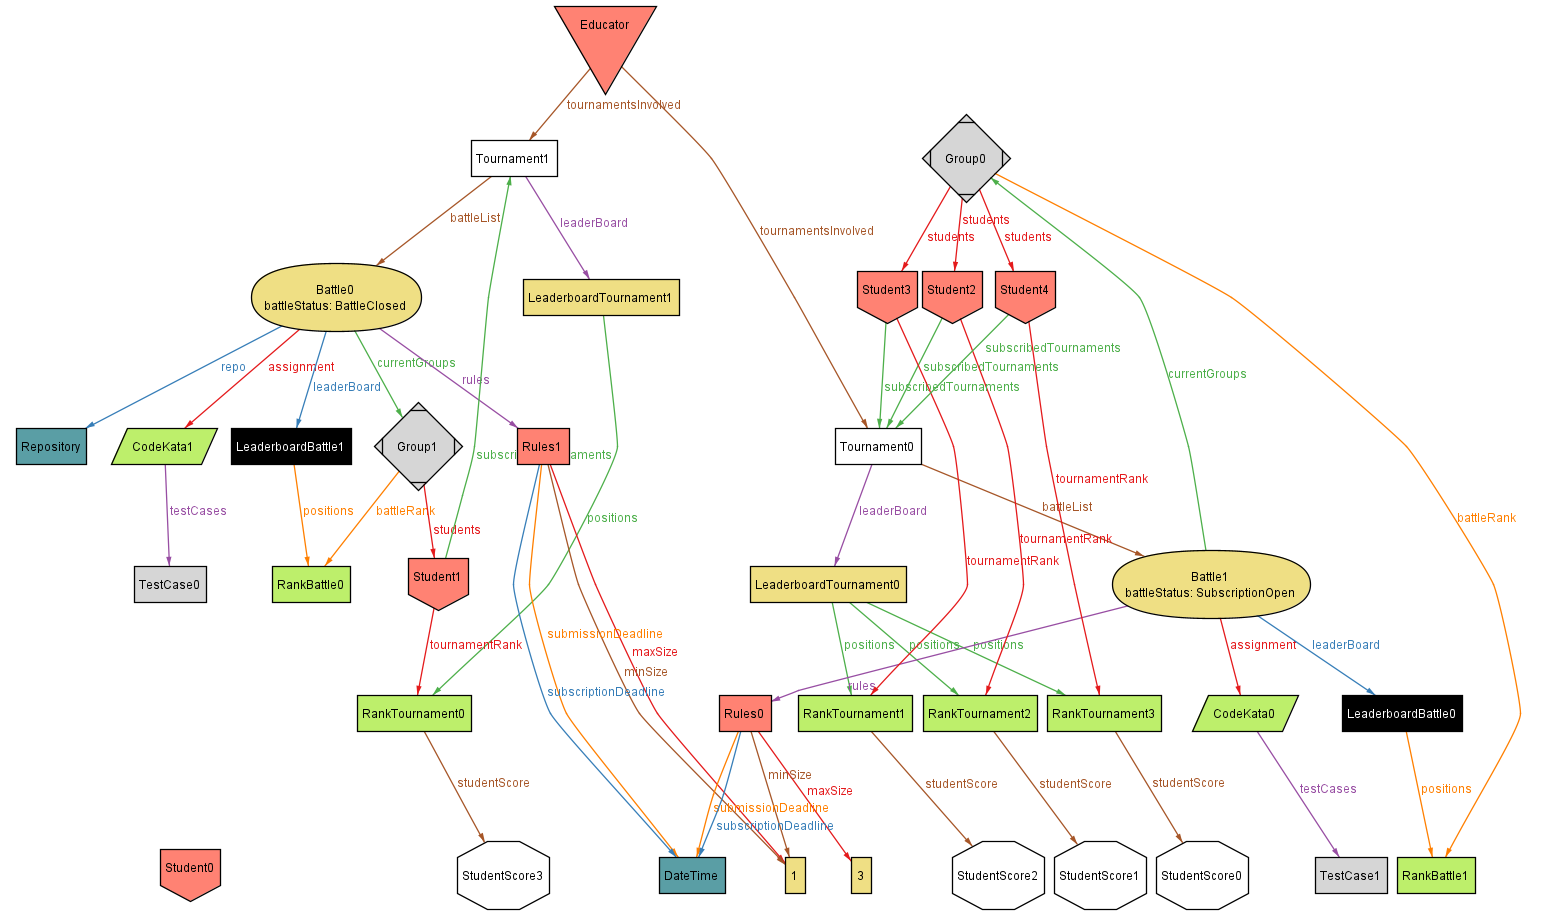
\includegraphics[width=1\linewidth]{misc/Images/AlloySims/showSomeRealistic.png}
            \caption{Simple world Alloy.}
        \end{center}
    \end{figure}
\end{sidewaysfigure}


\begin{figure}
    \centering
    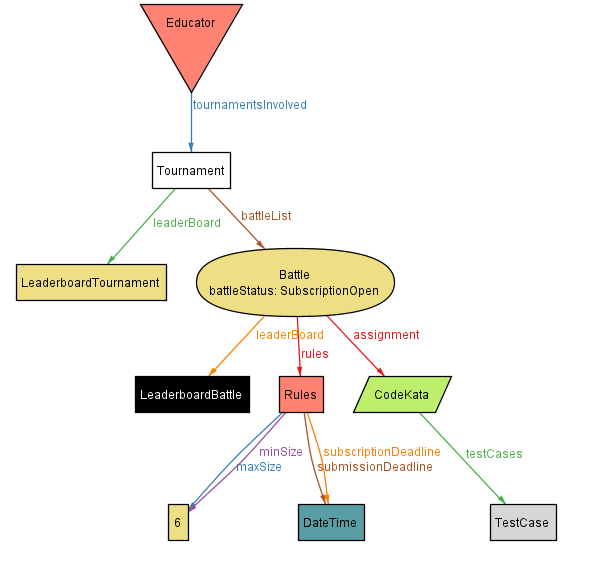
\includegraphics[width=1\linewidth]{misc//Images//AlloySims/noGroupBattle.png}
    \caption{Battle with no groups}
\end{figure}

\begin{sidewaysfigure}
    \begin{figure}[H]
        \begin{center}
            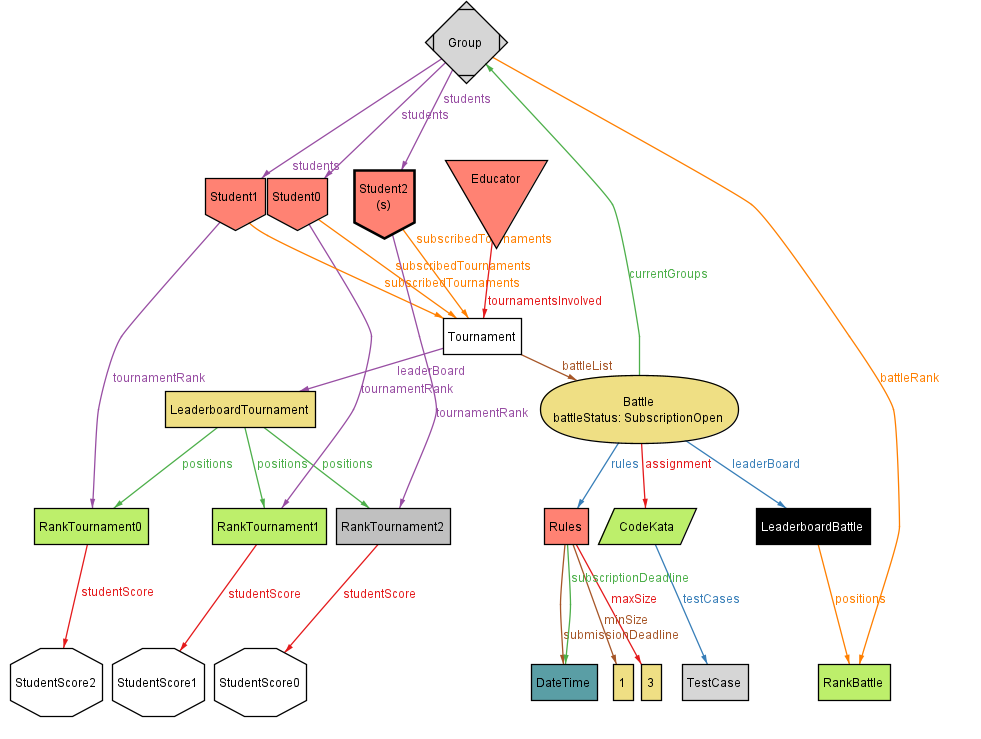
\includegraphics[width=1\linewidth]{misc//Images//AlloySims/joinNewBattle.png}
            \caption{Student joins a battle with a group}    
        \end{center}
    \end{figure}
\end{sidewaysfigure}


\begin{figure}
    \centering
    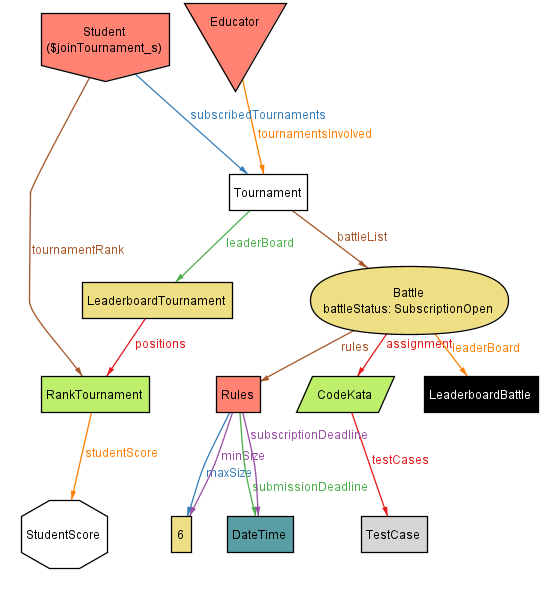
\includegraphics[width=1\linewidth]{misc//Images//AlloySims/joinTournament.png}
    \caption{Student joins a tournament}
    \label{fig:enter-label}
\end{figure}


%HERE IMAGES OF SIMULATIONS